\documentclass[main]{subfiles}

\begin{document}
\chapter{Visi\'on general del proyecto}
\label{chap:general}
En este cap\'itulo se describen brevemente las distintas partes que componen el proyecto de forma de que el lector se haga una idea general del mismo.\\

El esquema general de un cuadric\'optero se puede apreciar en la figura \ref{fig:cuad}\footnote{Las imágenes \ref{fig:cuad}, \ref{fig:cuad_roll}, \ref{fig:cuad_pitch} y \ref{fig:quad_theta} se basan en la original tomada de1 \url{http://www.isys.uni-stuttgart.de/}}. Se compone de dos ejes perpendiculares, en cuyos extremos se ubican los propulsores (motores y h\'elices). En dicha figura tambi\'en se observan las velocidades angulares de los motores ($\omega$), as\'i como las fuerzas ($T$) y torques ($M$) producidos por ellos. Tanto los torques como las fuerzas de los propulsores dependen de la velocidad angular de las h\'elices. Por dicho motivo, lo que se busca es actuar sobre los motores, variando su velocidad angular para realizar las distintas acciones de control.

\begin{figure}[h!]
\centering
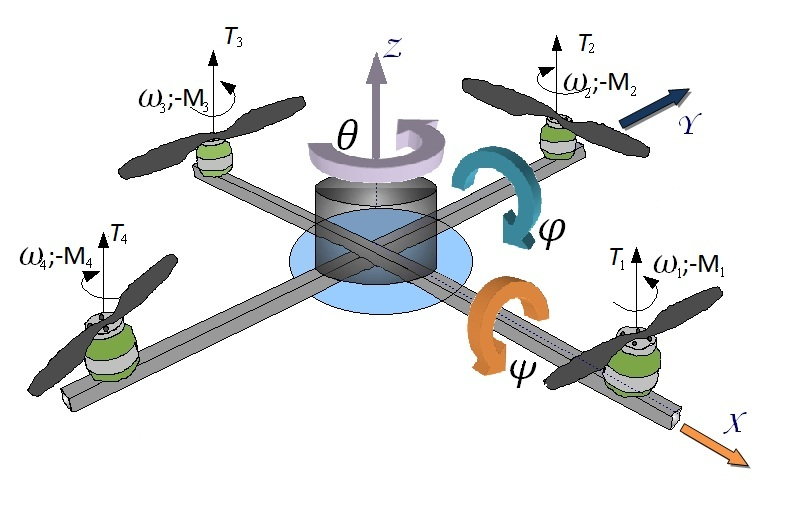
\includegraphics[scale=0.4]{./pics_general/quad_hov.jpg}
\caption{Esquema general de un cuadric\'optero}
\label{fig:cuad}
\end{figure}
\section{Acciones de control b\'asicas}
Existe una velocidad angular de los motores para la cual la fuerza total producida es igual al peso, esa velocidad angular permite que el cuadric\'optero permanezca suspendido con velocidad vertical nula, situaci\'on conocida como \emph{hovering}.\\ Si se aumenta uniformemente la velocidad angular de los motores la fuerza producida por los mismos supera al peso y el sistema se acelera hacia arriba. La reducción de la velocidad angular produce el efecto contrario.\\

\begin{figure}
\centering
\subfloat[Cambio en el \'angulo de Roll]{\label{fig:cuad_roll}
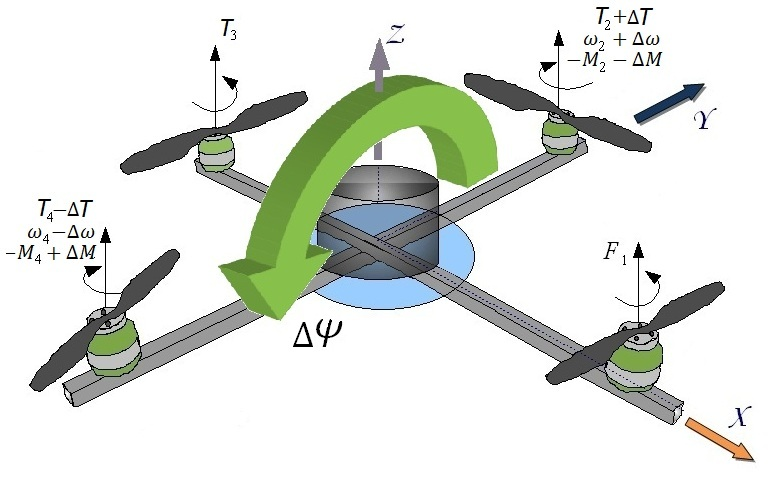
\includegraphics[scale=0.35]{./pics_general/quad_psi.png}}
\subfloat[Cambio en el \'angulo de Pitch]{\label{fig:cuad_pitch}
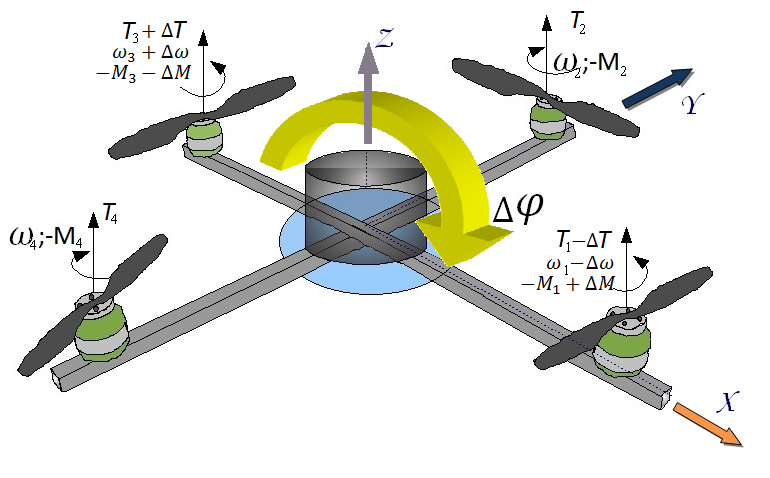
\includegraphics[scale=0.35]{./pics_general/quad_phi.png}}
\caption{}
\end{figure}

Para realizar una rotaci\'on se debe crear un desbalance entre los torques producidos por los motores. Si se desea aumentar el \'angulo de Roll ($\psi$), debe disminuirse la velocidad  angular del motor 4 y aumentar la del motor 2, manteniendo la fuerza neta igual a la fuerza necesaria para lograr el hovering. Esta situaci\'on se encuentra representada en la figura \ref{fig:cuad_roll}. Análogamente, para aumentar el \'angulo de Pitch debe aumentarse la velocidad angular del motor 3 y disminuir la velocidad angular del motor 1 (ver figura \ref{fig:cuad_pitch} ). Finalmente, si se desea aumentar el \'angulo de Yaw se debe disminuir la velocidad angular de los motores 1 y 3 y aumentar la de los motores 2 y 4, manteniendo la fuerza neta igual a la fuerza de hovering. Esta \'ultima situaci\'on es la presentada en la figura \ref{fig:quad_theta}.



\begin{figure}[!h]
\centering
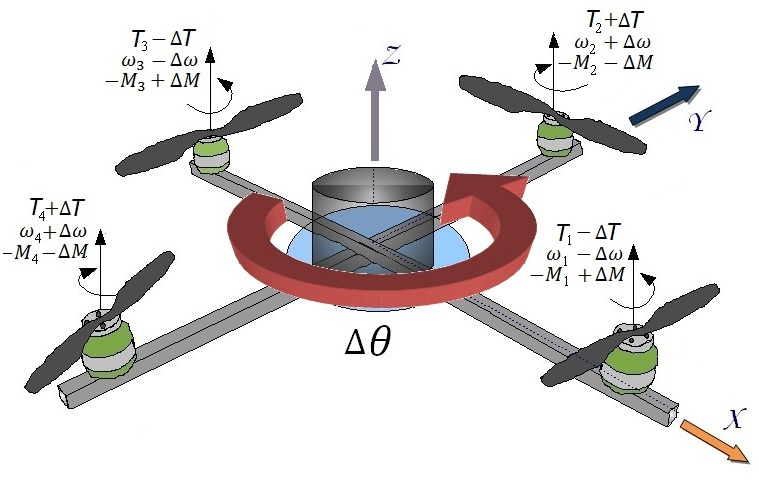
\includegraphics[scale=0.4]{./pics_general/quad_theta.jpg}
\caption{Cambio en el \'angulo de Yaw}
\label{fig:quad_theta}
\end{figure}
Las acciones de control descriptas anteriormente pueden ser combinadas de forma de lograr trayectorias m\'as complejas, gran parte de los cap\'itulos siguientes intentan explicar que acci\'on debe realizarse sobre cada motor para lograr diversos objetivos.

\section{Componentes del sistema y su interacci\'on}

A continuaci\'on se dar\'a una visi\'on general del sistema que se desea implementar. En la figura \ref{fig:esquema_gral_recortado} se presenta un diagrama de bloques de la plataforma física comercial adquirida, y en la figura \ref{fig:esquema_gral} el esquema general completo. En la proxima secci\'on se ver\'a en detalle el hardware utilizado.\\

\begin{figure}[h!]
  \centering
  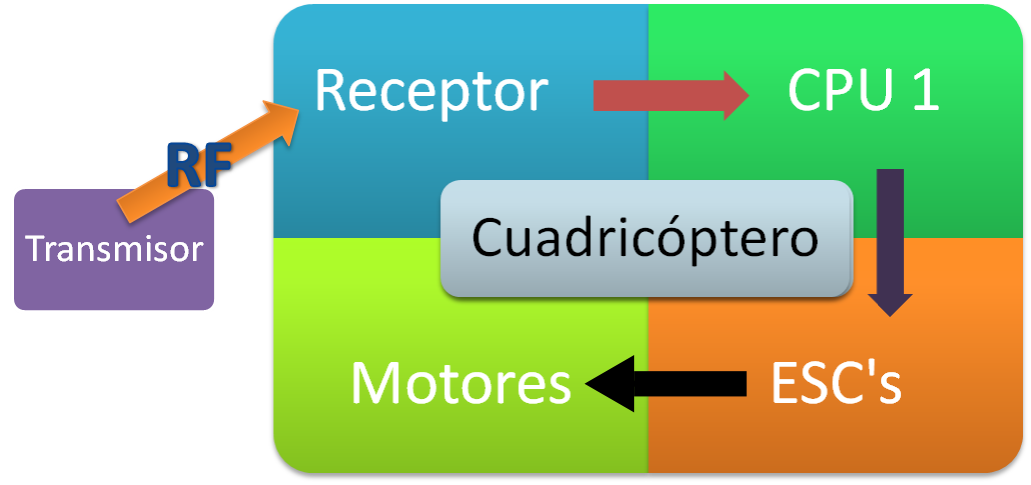
\includegraphics[width=.6\textwidth]{./pics_general/diagrama_gral_recortado_2.png}
  \caption{Esquema general de la plataforma física comercial}
  \label{fig:esquema_gral_recortado}
\end{figure}

La plataforma f\'isica elegida es un cuadric\'optero comercial radio controlado. El mismo cuenta con los elementos indispensables para poder volarlo manualmente: transmisor, receptor, CPU1, motores y ESCs\footnote{Electronic Speed Controller}. La soluci\'on adoptada agrega:
\begin{itemize}
\item IMU\footnote{Inertial Measurement Unit} y GPS: Sensores que permiten obtener una medida directa o indirecta de las variables de estado del sistema. 
\item CPU2: Es el centro del sistema de control a implementar, se encarga de procesar los datos de los sensores y de decidir la acci\'on de control a realizar. 
\item WiFi: Permite la comunicaci\'on con el mundo exterior de forma de facilitar la programaci\'on de los algor\'itmos y de modificar o agregar waypoints durante el vuelo. 
\item Switcheo: Una de las señales del receptor ser\'a utilizada para definir si el control de los motores estar\'a comandado por la CPU1 o por la CPU2. 
\end{itemize}

\begin{figure}[h!]
  \centering
  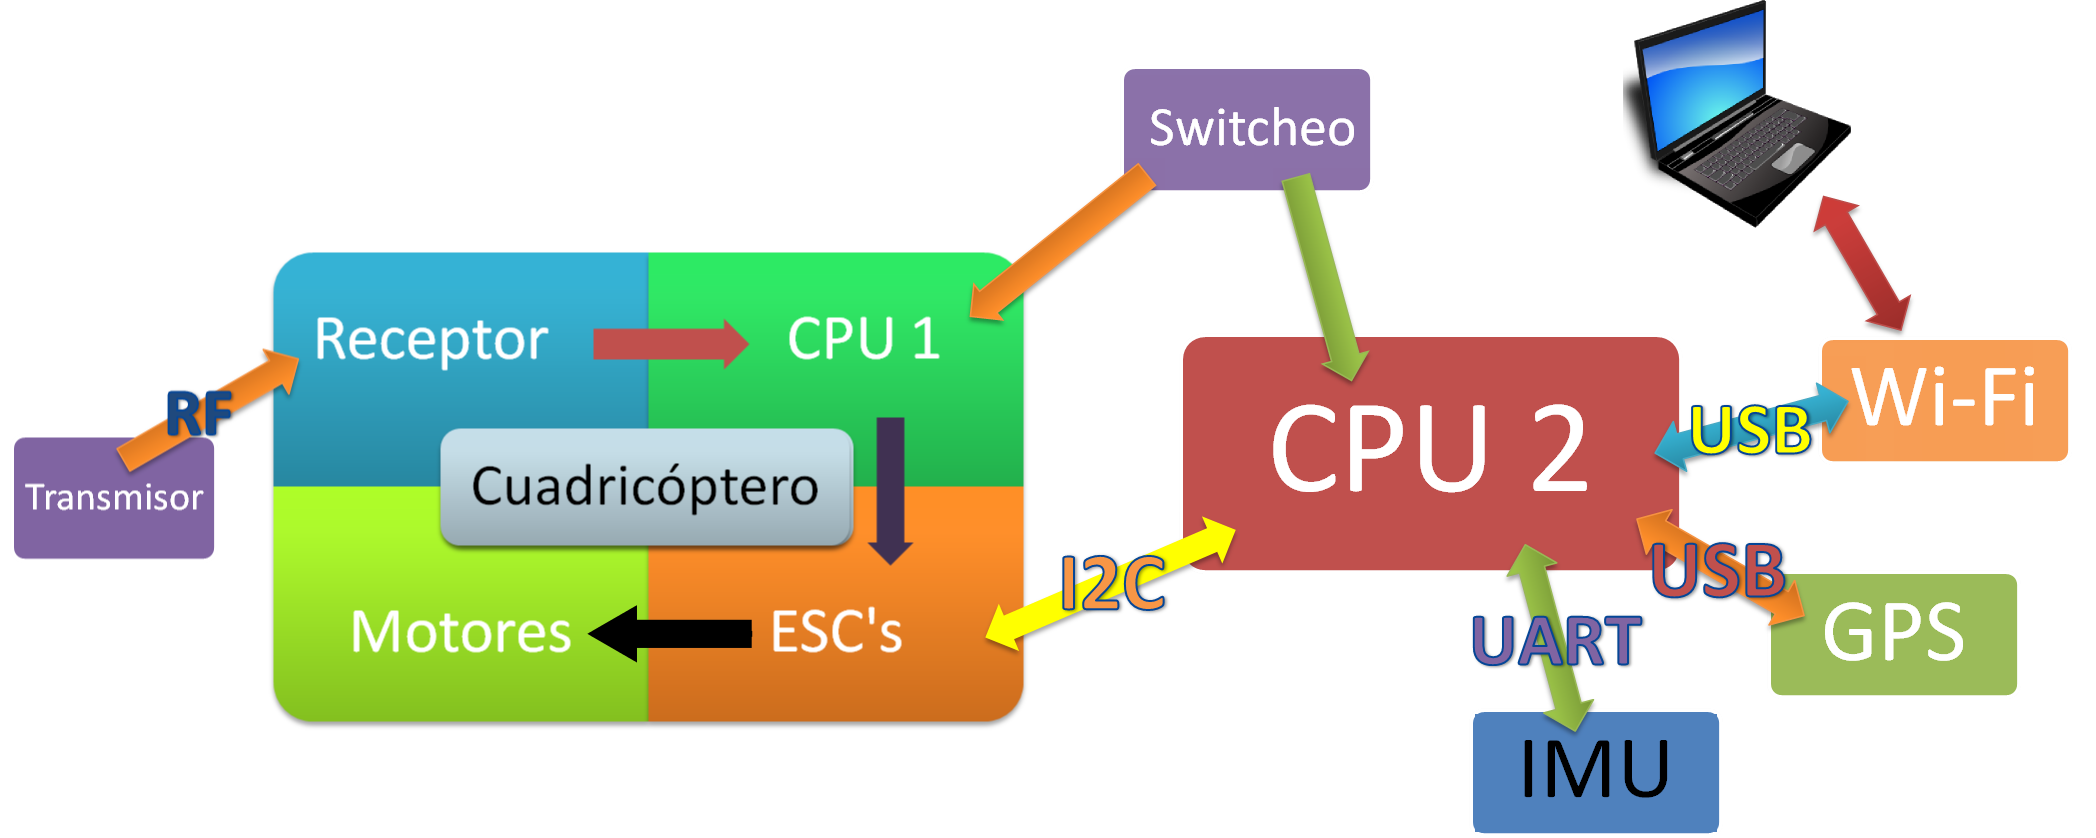
\includegraphics[width=1\textwidth]{./pics_general/diagrama_gral_2.png}
  \caption{Esquema general de interconexi\'on}
  \label{fig:esquema_gral}
\end{figure}

\end{document}